\section{Evaluation} \label{sec:evaluation}

We perform two kinds of evaluation a first one to compare the output of our system with the best results of the ASGRE challenge 2008, using automatic metrics provided in the challenge for comparison and the second one is a human evaluation we ask to two judges to select the best RE we will show that the judges prefered the system generated RE.

In order to perform the evaluation we take the development part of the TUNA corpus as test, it includes 80 RE for pictures of Furniture  and 60 RE for pictures of People.

\subsection{Automatic evaluation} \label{sec:automaticevaluation}

ACA ME GUSTARIA EXPLICAR MEJOR LAS METRICAS, Y EXPLICAR ALGO BASICO DE GRAPH

Using \puse~learned as described in Section~\ref{sec:learning} and running our algorithm 100 times, then we order from high to low the ouput of the system, so we have a list of RE with his respectives frequencies we call the most frequent RE SYS\_furniture\_1 for Furniture scenes and SYS\_People\_1 for People scenes, including the second more frequent we call SYS\_furniture\_2 and SYS\_people\_2 and so on until 20 including the 20th RE we call SYS\_furniture\_20 and SYS\_people\_20 then we execute the evaluation with the automatic metrics of the ASGRE challenge. 
In the challenge they calculate minimality, defined as the proportion of descriptions produced by a system
that are maximally brief, as per the original definition in Dale (1989). The Dice coefficient, used to compare the description produced by a system to the human-produced description on the same input domain. %Dice is estimated
MASI, a version of the Jaccard similarity coefficient proposed
by Passonneau (2006) which multiplies the similarity value by a monotonicity coefficient, biasing
the measure towards those cases where DS and
DH have an empty set difference. Intuitively, this
means that those system-produced descriptions are
preferred which do not include attributes that are
omitted by a human. Thus, two of our intrinsic measures assess Humanlikeness (Dice and MASI), while
Minimality reflects the extent to which an algorithm
conforms to brevity, one of the principles that has
emerged from the ASGRE literature.
Our results are comparable with the best results of the ASGRE challenge (The GRAPH system~\cite{KrahmerGRAPH}), but we also will show in the Section~\ref{sec:evaluation} that the RE generated by the system are more prefered than the humans ones.

In Table~\ref{Tabla_sis_1_20} we show the automatic metrics descripted below and comparison with our system the first more frequent and the one that includes the 20 more frequent RE.

\begin{table}[h!]
\begin{center}
\begin{tabular}{|l|c|c|c|c|}
\hline
%Figure & Model \puse &  Learning \puse & Random \puse &  Uniform \puse \\
	 	& 	DICE		&	MASI	&	A\_ACCURACY	&MINIMALITY	\\
\hline
GRAPH Furniture	& 	.80 		&	.59	&	.48		&	.0 	\\
GRAPH People 	& 	.72		&	.48	&	.28		&	.0	\\
\hline
SYS\_Furniture\_1	&	.79		&	.58	&	.43		&	.01	\\
SYS\_People\_1	&	.65		&	.37	&	.19		&	.0	\\
\hline
SYS\_Furniture\_20&	.87		&	.75  	&	.65		&	.01	\\
SYS\_People\_20	&	.81		&	.68	&	.60		&	.01	\\
\hline
\end{tabular}
%\vspace*{.1cm}
\caption{Comparison GRAPH and our system the more frequent and the first 20}
\label{Tabla_sis_1_20}
\end{center}
\end{table}
%\vspace*{-.9cm}
%Estos son los numeros que obtuve de accuracy para furniture (con estos hice el grafico)
%	GRAPH	OUR SYSTEM
%1	0.48	0.43
%5	0.48	0.5
%10	0.48	0.5375
%15	0.48	0.6
%20	0.48	0.65

% y estos para people
%	GRAPH	OUR SYSTEM
%1	0.28	0.19
%5	0.28	0.42
%10	0.28	0.47
%15	0.28	0.54
%20	0.28	0.6

In the Figurere~\ref{graficoPresicionFurniture} we can see that taking the first RE our system is a little lower than GRAPH but taking into account the first 5 more frequent RE given by the system our accuracy is the same of GRAPH, and taking 20 into account our system is as far better, for people in the Figure~\ref{graficoPresicionPeople} we can see that even taking less that 3 we have the same accuracy as GRAPH, and also if we take into account more RE the system is better.


\begin{figure}[ht]
\begin{minipage}{0.50\linewidth}
\centering
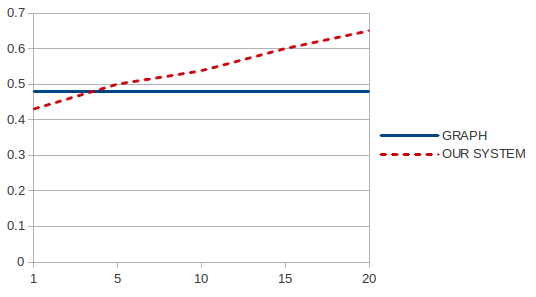
\includegraphics[width=\textwidth]{images/furniturePrec.png}
\caption{Comparison of accuracy of GRAPH and our system for furniture}
\label{graficoPresicionFurniture}
%\end{figure}
\end{minipage}
%\begin{figure}[ht]
\begin{minipage}{0.50\linewidth}
\centering
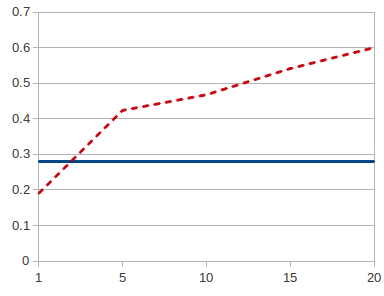
\includegraphics[width=\textwidth]{images/precP.png}
\caption{Comparison of accuracy of GRAPH and our system for people}
\label{graficoPresicionPeople}
\end{minipage}
\end{figure}

The dotted line is that represented by our system and the another is that represents the GRAPH performance.

Also we analyze the RE founded in the corpus that the system does not generate in a first frequency, and found that there were a 13.75\% in furniture that were not RE, those were underspecified sentences with does not identifies the target object. For people the proportion was lower just a 5.88\%. We saw that when a person used another word that was not taking into account in the annotation of the corpus, it was annotated as ``other'', and our system was not capable of generate ``other'' because it was not in the model.
In the table~\ref{error-furniture} there is a percentage of times in 100 runs that the system does not generates the RE given by the human for furniture, and as showed in Table~\ref{error-people} the human were more difficult to generate in the first 100 because the RE were longer the RE have less probability of occur. If the system does not generates the RE in 100 of runs does not mean that the system could not generate them, it just mean that the system need to be running more in order to generate this RE.\\


\begin{table}[h!]
\begin{center}
\begin{tabular}{|l|c|c|}
\hline
		& Count		& Percentage\\
\hline
It is not RE	&	11	&	13.75 \\
%		&	37	&	46.25\% \\
Contains ``other''	&	6	&	7.50 \\
\hline
SYS does not generated the RE in 100 runs	&	8	&	10.00 \\
SYS generated but not with higher frequency	&	18	&	22.5 \\
\hline
\end{tabular}
%\vspace*{.1cm}
\caption{Clasification of RE that the system could not generates or generates with low frequency for Furniture}
\label{error-people}
\end{center}
\end{table}
%\vspace*{-.4cm}

\begin{table}[h!]
\begin{center}
\begin{tabular}{|l|c|c|}
\hline
			& Count		& Percentage\\
\hline
It is not RE		&	4	&	5.88 \\
Contains ``other''	&	6	&	8.82 \\
\hline
SYS does not generated the RE in 100 runs	&	17	&	25.00 \\
SYS generated but not with higher frequency	&	28	&	41.18 \\
%BIEN			&	13	&	19.12\% \\

\hline
\end{tabular}
%\vspace*{.1cm}
\caption{Clasification of RE that the system could not generates or generates with low frequency for People}
\label{error-furniture}
\end{center}
\end{table}
%\vspace*{-.4cm}
\subsection{Human evaluation} \label{sec:humanevaluation}

We aisle the RE that our system gives another RE with more frequency it is that not coincides with the one given by the human in the corpus, and with those realize a human evaluation in order to see if the RE produced by the system are prefered by human than the RE produced by humans. Two judges fluent or natural speakers of English were asked to select the best of each pair of RE.

We have 43 scenes of furniture (from 80) and 55 scene of people (from 68), for which of them we manually realize the referring expressions (including the properties given as results by our algorithm) and ask people to evaluate which one is a RE it is that univocally identifies the target object and wich one is better in sense that will be more usefull for a human who is not seeing the red box to identify the object. For do it we prepare a webpage with each of the pictures and 2 choices randomly ordered human and system RE. Out goal is to try to show if RE produced by our system are at less as good as the produced by human, and also we will show that they are even better.

%\begin{table}[h!]
%\begin{center}
%\begin{tabular}{|c|c|c|c|}
%\hline
%           & Agree in & Not agree & Total\\
%\hline 
%Furniture & 25       & 18        & 43 \\
%People    & 25       & 30        & 55 \\
%Total     & 50       & 48        & 98 \\
%\hline
%\end{tabular}
%\caption{Agree between judges} 
%\label{agree-judges}
%\end{center}
%\end{table}

%esta tabla no ayuda...no se que decir, no se como justificar que no coincidan...
%In the Table~\ref{agree-judges} we can see that the both judges choice the same RE 25 times for Furniture and 25 times for People, 

\begin{table}[h!]
\begin{center}
\begin{tabular}{|c|c|c|c|c|}
\hline
Judge    & Human choice & System choice  & Human choice & System choice \\
	 &    Furniture &    Furniture   &    People    &    People \\
\hline 
Judge1   & .23       & .77      & .45  & .55  \\
Judge2   & .26       & .73      & .41  & .59  \\
\hline
\end{tabular}
%\vspace*{.1cm}
\caption{Porcentage of system versus human selected choices for each judge} 
\label{system-versus-human}
\end{center}
\end{table}
%\vspace*{-.9cm}
In the Table~\ref{system-versus-human} you can see the judges selected more the RE generated by our system than the human RE.

%\begin{table}[h!]
%\begin{center}
%\begin{tabular}{|c|c|c|c|}
%\hline
%Judge    & Human choice & System choice & Total\\
%\hline 
%Judge1 & 25       & 30        & 55 \\
%Judge2    & 23       & 32        & 55 \\
%\hline
%\end{tabular}
%\caption{System versus human selected choice for People} 
%\label{system-versus-human-people}
%\end{center}
%\end{table}

%In the case of pictures of people you can see in the Table~\ref{system-versus-human-people} that the judges selected more RE generated by our system but the diference in not very significant.

\begin{table}[h!]
\begin{center}
\begin{tabular}{|c|c|c|c|c|c|}
\hline
           & System & System (\%) & Human & Human (\%) & Total\\
\hline
Furniture & 23  & .92 &  2 & .08  & 25 \\
People    & 16  & .64 & 9  & .36 & 25 \\
\hline
Total     & 39  & .78    & 11 & .22 & 50  \\
\hline
\end{tabular}
%\vspace*{.1cm}
\caption{Coincidences between judges, the system is the prefered the 78\% of times} 
\label{system-better}
\end{center}
\end{table}
%\vspace*{-.9cm}
Taking into account just the coincidences between jugdes the Table~\ref{system-better} shows the percentage of their preference, they prefered the system in 78\% of times.

Sometimes comparison was unfair because human gives a RE that includes relation that were not annotated so, the system haven't the posibility of produce them. A point in favor of the system is that sometimes the human did an underespecified RE and the system has a better one.\\


Sometimes judges choices the same RE for example in Figure~\ref{smallBlueFan1} the RE given by the human was underspecified, so they choice the system one because was a RE. Another times just RE given by the system was intuitivelly less complex than the human one like in Figure~\ref{smallBlueFan} where RE of the system was ``small blue fan'' and the human RE was ``bottom row, blue fan''.
\begin{figure}[ht]
\begin{minipage}{0.50\linewidth}
\centering
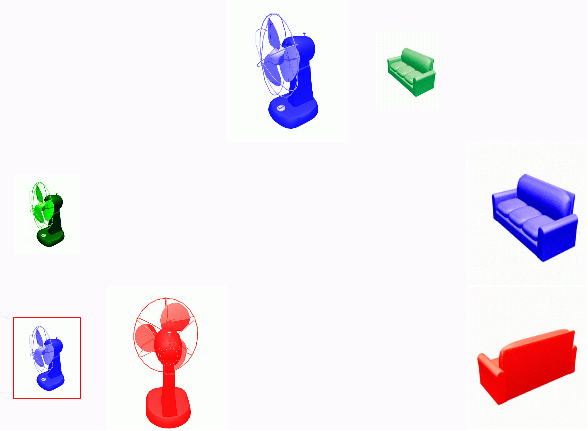
\includegraphics[width=\textwidth]{images/smallBlueFan1.jpg}
\caption{TUNA corpus furniture scene}
\label{smallBlueFan1}
\end{minipage}
\begin{minipage}{0.50\linewidth}
\centering
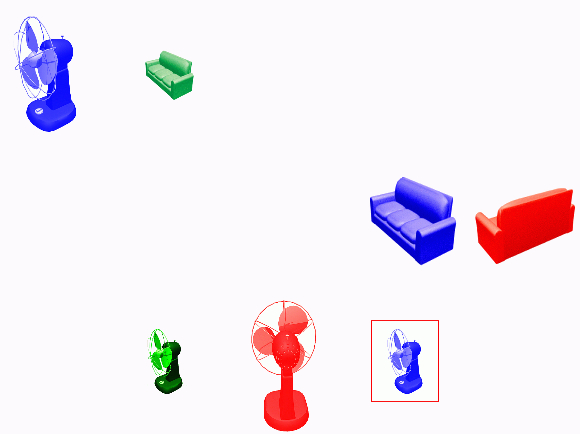
\includegraphics[width=\textwidth]{images/smallBlueFan.jpg}
\caption{TUNA corpus furniture scene}
\label{smallBlueFan}
\end{minipage}
\end{figure}

Sometimes the judges choice the human RE for example in Figure~\ref{largeGreyChair} the
system RE was ``large grey chair facing away'' and the human RE was ``the top left grey chair''.

\begin{figure}[ht]
%\begin{minipage}{0.50\linewidth}
\centering
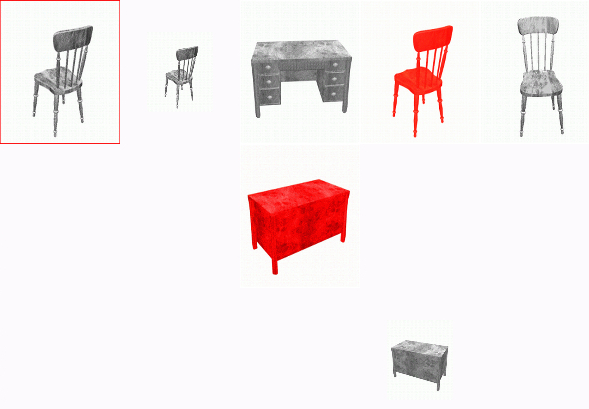
\includegraphics[width=0.8\textwidth]{images/largeGreyChair.jpg}
\caption{TUNA corpus furniture scene}
\label{largeGreyChair}
\end{figure}

\begin{figure}[ht]
\begin{minipage}{0.50\linewidth}
\centering
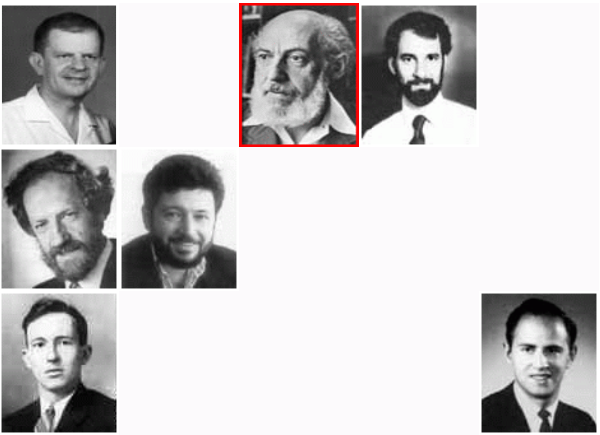
\includegraphics[width=\textwidth]{images/s28t25.png}
\caption{Scene used during the collection of the TUNA corpus. The human RE was ``man in middle row, on the right'', and the system ``the man with a beard wearing glasses''. Judges prefer}
\label{s28t25}
%\end{figure}
\end{minipage}
%\begin{figure}[ht]
\begin{minipage}{0.50\linewidth}
\centering
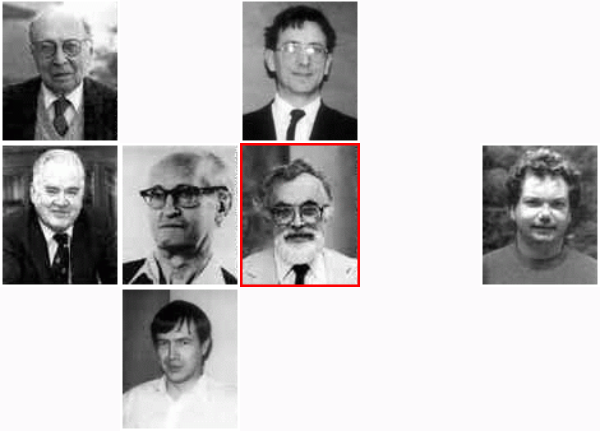
\includegraphics[width=\textwidth]{images/s307t21.png}
\caption{Scene used during the collection of the TUNA corpus. The human RE was ``man with white beard'', and the system ``the man with a beard ''. Judges prefer}
\label{s307t21}
\end{minipage}
\end{figure}



EN HUMAN EVALUATION AGREGAR CASOS EN LOS QUE LOS JUECES CONSISTENTEMENTE ELIGIERON LA EXPRESION DE LA PERSONA Y CASOS EN LOS QUE LOS JUEVES ELIGIERON CONSISTENTEMENTE EXPRESIONES HUMANAS. DAR UNA IDEA DE PORQUE LAS EXPRESIONES DEL SISTEMA SON A VECES MEJORES Y PORQUE A VECES LAS DE LOS HUMANOS SON MEJORES (E.G. DEPENDENCIA ENTRE X E Y)
